\documentclass[../main/main.tex]{subfiles}

\begin{document}

\onlyinsubfile{%

}

% ==================================================================
% Section : Modern Interpretation of the specifications
% ==================================================================
\section{Modern Interpretation of the specifications}

\begin{frame}{Modern Interpretation of the specifications - Outline}
  \tableofcontents[currentsection, hideothersubsections]
\end{frame}
% ==================================================================

% ==================================================================
\subsection{Standart Control Architecture}

\begin{frame}{Standart Control Architecture}
  \centering
  \begin{overprint}
    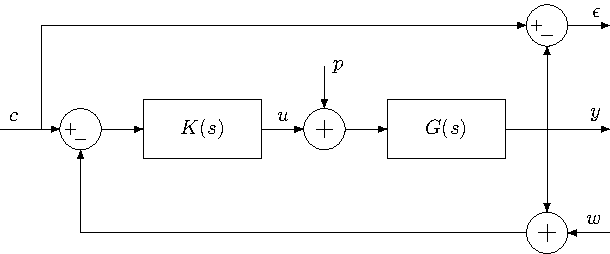
\includegraphics[width=1.0\textwidth, height=0.9\textheight, keepaspectratio]{h-infinity-variables}
    \onslide<1>
    \[
      \epsilon(s) = \overbrace{T_{c\rightarrow \epsilon}}^{S} c(s) +
      \overbrace{T_{p\rightarrow \epsilon}}^{GS} p(s) +
      \overbrace{T_{w\rightarrow \epsilon}}^{T} w(s)
    \]
    \[
      u(s) = \underbrace{T_{c\rightarrow u}}_{KS} c(s) +
      \underbrace{T_{p\rightarrow u}}_{T} p(s) +
      \underbrace{T_{w\rightarrow u}}_{-KS} w(s)
    \]

    \onslide<2>
    \[ S(s) = \frac{1}{1+G(s)K(s)} = \text{ Sensibility Tranfert Function}\]
    \[ T(s) = \frac{G(s)K(s)}{1+G(s)K(s)} = \text{ Transmissibility Function}\]
    \[ S(s) + T(s) = 1 \rightarrow \text{Closed loop functions are linked!}\]
  \end{overprint}
\end{frame}
% ==================================================================

% ==================================================================
\subsection{Classical Specifications}

\begin{frame}{Classical Specifications - Time domain}
  \begin{itemize}
  \item \textbf{Stability} \onslide<2>{\(S(s)\) \(T(s)\) \(K(s)S(s)\) \(G(s)S(s)\)}
  \item \textbf{Reference tracking} \onslide<2>{\(S(s) = T_{c \rightarrow \epsilon}\)}
    \begin{itemize}
    \item Precision for a specific input - Zero static error
    \item Overshoot, oscillations
    \item Speed: time response, rejection
    \end{itemize}
  \item \textbf{Disturbances rejection} \onslide<2>{\(G(s) S(s) = T_{p \rightarrow \epsilon}\)}
  \item \textbf{Measurement noise filtering} \onslide<2>{\(T(s) = T_{w \rightarrow \epsilon}\)}
  \item \textbf{Small command amplitude} \onslide<2>{\(K(s) S(s) = T_{c \rightarrow u}\)}
  \item Controller implementation
  \end{itemize}
\end{frame}
% ==================================================================

% ==================================================================
\subsection{Modern Specifications}

\begin{frame}{Modern Specifications - Closed Loop TF}
  \centering
  \begin{itemize}
  \item With \(H_{\infty}\), we work with closed-loop tranfert functions
  \item We have to translate each specification into the shape that the
    transfert function associated needs to have
  \item Basically, there is 4 tranfert functions that we will use
  \end{itemize}

  \begin{tabular}{| c | c |}
            \hline
            \textbf{Specifications}     & \textbf{Tranfert Function}         \\ \hline
            Stability                   & \(S\) \(T\) \(KS\) \(GS\)                  \\ \hline
            Reference tracking          & \(S(s) = T_{c \rightarrow \epsilon}\)      \\ \hline
            Disturbances rejection      & \(G(s) S(s) = T_{p \rightarrow \epsilon}\) \\ \hline
            Measurement noise rejection & \(T(s) = T_{w \rightarrow \epsilon}\)      \\ \hline
            Small command amplitude     & \(K(s) S(s) = T_{c \rightarrow u}\)      \\ \hline
  \end{tabular}
\end{frame}
% ==================================================================

\begin{frame}{Reference tracking}
  
  \stitle{Influence of the signal \(c(t)\) on the signal \(\epsilon(t)\)}

  \begin{columns}[T]
    \begin{column}{0.5\textwidth}
      \begin{tcolorbox}[size=small, top=4pt, colback=blue!5!white,colframe=blue!75!black,title=2 states]
        \begin{itemize}
        \item Transiant state
        \item Steady state
        \end{itemize}
      \end{tcolorbox}
    \end{column}
    \begin{column}{0.5\textwidth}
      \begin{tcolorbox}[size=small, top=4pt, colback=blue!5!white,colframe=blue!75!black,title=Multiples input signals]
        \begin{itemize}
        \item Step signal
        \item Ramp
        \item Sinusoidal
        \end{itemize}
      \end{tcolorbox}
    \end{column}
  \end{columns}
\end{frame}

\begin{frame}{Reference tracking - Steady State}
  \(c(t) = A \Gamma(t) \overset{\mathcal{L}}{\Longrightarrow} c(s) = \frac{A}{s\)}

  We want \(\lim_{t\rightarrow\infty}\epsilon(t) = 0\) with \(\epsilon(s) = T_{c\rightarrow\epsilon}(s)c(s\)

  \begin{tcolorbox}[size=small, top=4pt, colback=blue!5!white,colframe=blue!75!black,title=Final value theorem]
    If \(\lim_{t\rightarrow\infty}\) has a finite limit then \(\lim_{t\rightarrow\infty} = \lim_{s\rightarrow 0}s \mathcal{F}(s\)
  \end{tcolorbox}
  \vspace{-2em}
  \begin{align*}
    \lim_{t\rightarrow\infty}\epsilon(t) & = \lim_{s\rightarrow 0}s \epsilon(s) = \lim_{s\rightarrow 0} s T_{c\rightarrow\epsilon}(s) c(s)\\
    & = \lim_{s\rightarrow 0} s T_{c\rightarrow\epsilon}(s) \frac{A}{s} = \lim_{s\rightarrow 0} A T_{c\rightarrow\epsilon}(s) = 0
  \end{align*}

  \begin{tcolorbox}[size=small, top=4pt,
    colback=red!5!white,colframe=red!75!black,title=If we want to have no
    tracking error on step input]
    \(T_{c\rightarrow\epsilon}(s)\) must contains a zero at zero
  \end{tcolorbox}
\end{frame}

\begin{frame}{Reference tracking - Transiant State}
  We want \(\epsilon(t) = c(t) - y(t)\) small \(\forall t\)

  \begin{tcolorbox}[size=small, top=4pt,
    colback=blue!5!white,colframe=blue!75!black,title=Duality Time -Frequency]
    \[
      \epsilon(t) \text{ small } \forall t \Longleftrightarrow \epsilon(j\omega)
      \text{ small } \forall \omega
    \]
  \end{tcolorbox}

  $\epsilon \text{ small }: \epsilon \in \mathcal{E} = \left\{ \epsilon\text{ so that} \abs{\epsilon(j\omega)} \le \epsilon_{\text{sup}}A, \forall \omega \right\}$

  \begin{equation*}
    \forall \omega, \abs{\epsilon(j\omega)} \le \epsilon_{\text{sup}}A \Leftrightarrow \forall \omega, \abs{T_{c\rightarrow\epsilon}(j\omega) \frac{A}{j\omega}} \le \epsilon_{\text{sup}}A
  \end{equation*} 

  \begin{tcolorbox}[size=small, top=4pt,
    colback=red!5!white,colframe=red!75!black,title=If we want small error
    during transiant state]
    \[
      \forall \omega, \abs{T_{c\rightarrow\epsilon}(j\omega)} \le \epsilon_{\text{sup}}\abs{j\omega}
    \]
  \end{tcolorbox}
\end{frame}


\begin{frame}{Weighting Functions}
  \centering
  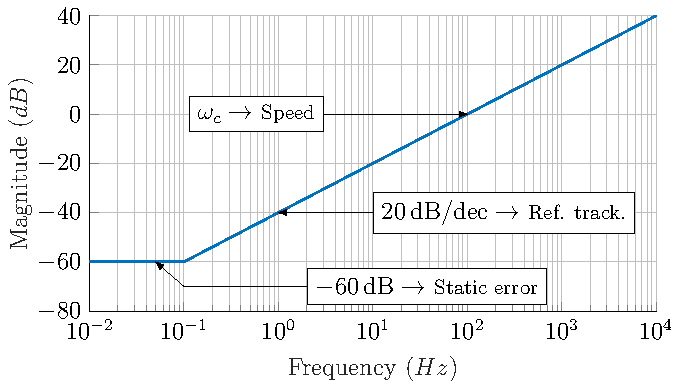
\includegraphics[width=1.0\textwidth, height=0.9\textheight, keepaspectratio]{contr_W1_first}
\end{frame}


\begin{frame}{Weighting Functions}
  \centering
  \begin{columns}
    \begin{column}{0.5\textwidth}
      There are 3 weighting functions used to ''\emph{shape}'' the CL TF:
      \begin{itemize}
      \item \(T_{c \rightarrow \epsilon} \Longrightarrow W1\)
      \item \(T_{p \rightarrow \epsilon} \Longrightarrow W1 W3\)
      \item \(T_{w \rightarrow \epsilon} \Longrightarrow W2 W3\)
      \item \(T_{c \rightarrow u} \Longrightarrow W2\)
      \end{itemize}
    \end{column}
    \begin{column}{0.5\textwidth}
      \begin{tcolorbox}[size=small, top=4pt,
        colback=red!5!white,colframe=red!75!black,title=Global \(\hinf\) criteria]
        \vspace{-1em}
        \[
          \begin{Vmatrix}
            W_1 S & W_1 GS W_3 \\
            W_2 KS & W_2 T W_3
          \end{Vmatrix}_{\infty} < 1
        \]
      \end{tcolorbox}
    \end{column}
  \end{columns}
  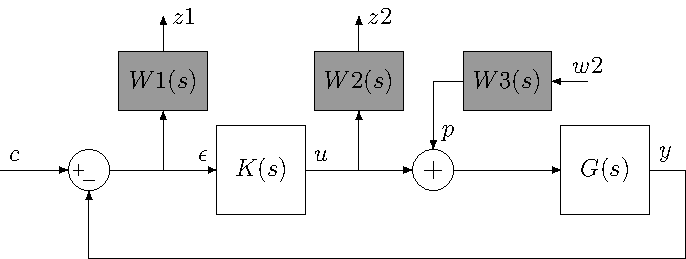
\includegraphics[width=1.0\textwidth, height=0.9\textheight, keepaspectratio]{critere_4_blocs}
\end{frame}


\begin{frame}{Weighting Functions - What can we ''\emph{shape''} ?}
  \centering
  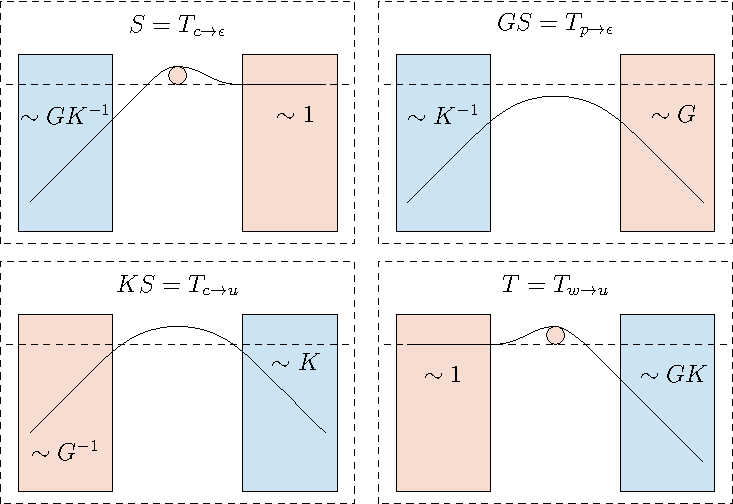
\includegraphics[width=1.0\textwidth, height=0.9\textheight, keepaspectratio]{contraintes}
\end{frame}


% ==================================================================
\subsection{H-infinity Synthesis Methodology}

\begin{frame}{\(\hinf\) Synthesis Methodology}
  \centering
  \begin{itemize}
  \item Iterative
  \item Before choosing the weighting functions
  \end{itemize}
  \begin{tcolorbox}[size=small, top=4pt,
    colback=blue!5!white,colframe=blue!75!black,title=This is my own methodology]
    Use it at your own risk!
  \end{tcolorbox}
\end{frame}

\begin{frame}{\(\hinf\) Synthesis Methodology - W1}
  \centering
  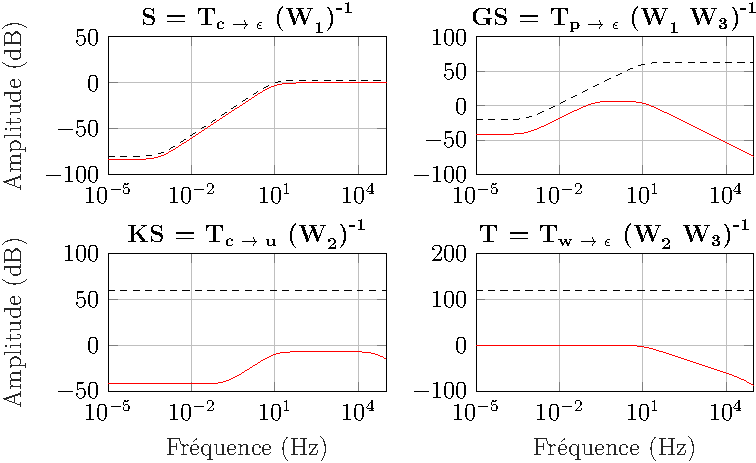
\includegraphics[width=1.0\textwidth, height=0.8\textheight, keepaspectratio]{contr_step_1}
\end{frame}

\begin{frame}{\(\hinf\) Synthesis Methodology - W2}
  \centering
  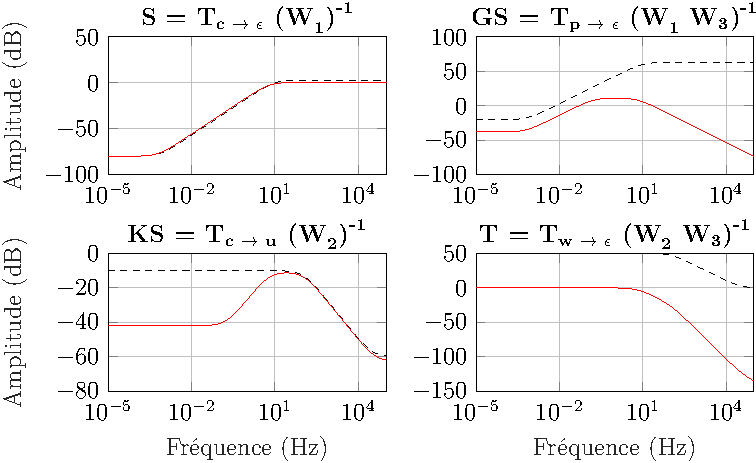
\includegraphics[width=1.0\textwidth, height=0.8\textheight, keepaspectratio]{contr_step_2}
\end{frame}

\begin{frame}{\(\hinf\) Synthesis Methodology - W3}
  \centering
  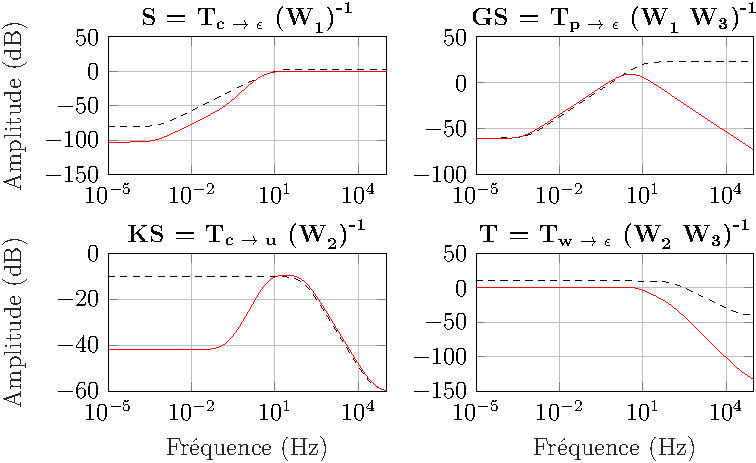
\includegraphics[width=1.0\textwidth, height=0.8\textheight, keepaspectratio]{contr_step_3}
\end{frame}
% ==================================================================


\end{document}

